\chapter{Estado del Arte}
\thispagestyle{empty}

En el campo del aprendizaje automático, el tema de la estimación de la distancia en fotografías faciales ha ganado recientemente mucha atención. Se puede observar en la Figura \ref{fig5} la cantidad de publicaciones existentes en la base de datos Scopus \footnote{Las búsquedas se pueden consultar en el apéndice} que hacen referencia a la estimación del SCD. Hay 430 publicaciones registradas desde 1992.

El número de publicaciones relacionadas con este tema, va aumentando a lo largo del tiempo, llegando a obtener un mayor número de publicaciones en 2020. Pese al aumento de publicaciones en este ámbito, es a partir del 2015 cuando se empiezan a aplicar las técnicas de deep learning. Este aumento está relacionado con los avances tecnológicos que permiten aplicar nuevas técnicas y conocimientos. 

\begin{figure}[h]
	\centering
	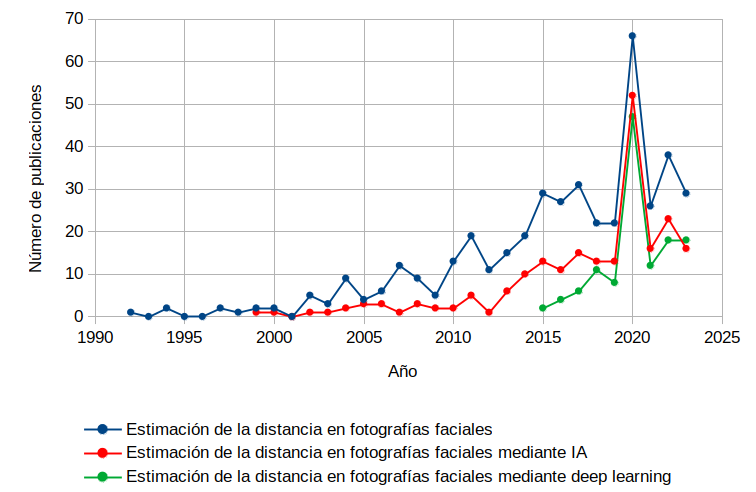
\includegraphics[scale=0.45]{imagenes/cap3/grafica_scopus3.png}
	\caption{Número de publicaciones, en Scopus, relacionadas con la estimación de la distancia en fotografías faciales en función del año de publicación}
	\label{fig5}
\end{figure}

\section{Primeros enfoques}

El primer método utilizado para abordar la estimación métrica del SCD fue propuesto por \cite{28}, se basa en el uso de un conjunto de puntos de referencia de la cara para estimar la pose y la distancia a la cámara en distancias desde 10 cm hasta 3 m. El proceso consiste en, entrenar un modelo de regresión para predecir la distancia entre la cámara y la cara, utilizando un conjunto de imágenes 3D de caras humanas con sus respectivos puntos de referencia faciales (se observa que estas referencias no varían drásticamente entre individuos, sino que se agrupan en 'clusters'). Dicho conjunto de datos 3D solo contiene vistas de frontales y de perfil 3/4. 

Dada una imagen 2D de una cara desconocida, se identifican los puntos de referencia faciales y mediante el algoritmo EPnP \cite{29}, junto con la suposición de que las referencias no varían mucho entre individuos, se infiere la pose 3D de la cara y se utiliza el modelo de regresión previamente entrenado para predecir el valor de la distancia a la cámara.

Algunas de las limitaciones asociados a este primer método son: el uso de un conjunto de datos 3D (no siempre tendremos disponibles imágenes 3D para el entrenamiento), la combinación de diferentes longitudes focales en el mismo dataset o el reconocimiento manual de los puntos de referencia faciales

Posteriormente, \cite{30} propuso un método que no necesitaba la reconstrucción 3D ni la anotación manual de los puntos de referencia de la imagen. Este método utiliza un conjunto de datos llamado Caltech Multi-Distance Portraits (CMDP), compuesto de 53 retratos individuales desde 7 distancias distintas entre 60 cm y 480 cm, para entrenar el modelo. Todas las imágenes del conjunto de datos fueron anotadas manualmente con 55 marcas faciales. 

El método se basa en dos fases: primero, la identificación automática de los puntos de referencia faciales, y después, la estimación de la distancia mediante regresión.

Este nuevo enfoque, a pesar de mejorar lo que previamente se había hecho, sigue teniendo algunas limitaciones como el recorte de las imágenes (pérdida de resolución) o la única vista frontal.

Existen otros métodos que estiman el SCD a partir de características anatómicas como el tamaño de la cara \cite{32}, la distancia de los ojos \cite{33} o una combinación de ambos \cite{34}.

\section{MediaPipe Iris}

MediaPipe Iris \footnote{https://blog.research.google/2020/08/mediapipe-iris-real-time-iris-tracking.html} es un modelo de aprendizaje automático, creado por investigadores de Google, capaz de seguir puntos de referencia (iris, pupila y contornos del ojo) usando una cámara RGB, en tiempo real, y sin necesidad de ningún hardware especializado. A través de los puntos de referencia del iris, el model es capaz de determinar la distancia métrica entre el sujeto y la cámara.

El modelo se basa en el diámetro horizontal del iris del ojo humano, que se mantiene relativamente constante en un rango de 11.7±0.5 mm en una amplia población, esto junto con algunos simples argumentos geométricos, permiten la posibilidad de estimar el SCD.

Este modelo requiere de unas condiciones, que además, son sus principales limitaciones. El modelo solo puede ser usado cuando: existen datos EXIF disponibles; son imágenes frontales donde el iris es visible; y los individuos están a menos de 2m de la posición de la cámara.



\section{PerspectiveX}

PerspectiveX fue el método propuesto por Stephan en \cite{31} para la estimación del SCD en fotografías faciales con el fin de mejorar el proceso de superposición craneofacial.

Este método se basa en la localización de una característica anatómica, la longitud de la fisura palpebral entre dos marcas precisas y fácilmente determinables. Se utiliza este rasgo anatómico debido a que: es fácilmente visible en vista frontal e incluso en el lado más cercano a la cámara si la cabeza está girada; está definida por dos puntos de referencia muy precisos; tiene una variación muy ajustada, debido a restricciones evolutivas; es una característica facial relativamente grande, por lo que, minimiza el impacto de los errores en comparación con otras características faciales invariantes como el diámetro del iris; tiene una distribución normal que reduce el error de predicción a la mitad.

Además de la fisura palpebral, PerspectiveX necesita conocer el tipo de cámara y la longitud focal de las lentes, que se pueden extraer siempre de imágenes electrónicas usando lectores EXIF disponibles en internet. El tipo de cámara es necesario para obtener las especificaciones de píxeles.

Finalmente, la estimación del SCD se realiza mediante la siguiente fórmula:

\begin{equation}
	SCD = f (1+\frac{A}{x \cdot y})
\end{equation}

donde: $f$, es la longitud focal de las lentes (mm); $A$, es la longitud real de la fisura palpebral (mm); $x$, es la longitud de la fisura palpebral en la foto (píxeles); $y$, son las especificaciones del tamaño del píxel del receptor de imagen (mm)

Al no disponer de la longitud real de la fisura palpebral, se utiliza el valor medio de un conjunto de individuos agrupados por sexo y edad, ya que, sabemos que la longitud varía muy poco debido a restricciones evolutivas.

Este método permite una precisa estimación del SCD para una longitud focal conocida. Sin embargo, este método posee unas limitaciones como: el requerimiento de interacción manual para anotar los puntos de referencia faciales; y que no tiene en cuenta las rotaciones de cabeza de más de 30º.

\section{FacialSCDnet}


